 %%%%%%%%%%%%%%%%%%%%%%%%%%%%%%%%%%%%%%%%%%%%%%%%%%%%%%%%%%%%%%%%%%%%
%% I, the copyright holder of this work, release this work into the
%% public domain. This applies worldwide. In some countries this may
%% not be legally possible; if so: I grant anyone the right to use
%% this work for any purpose, without any conditions, unless such
%% conditions are required by law.
%%%%%%%%%%%%%%%%%%%%%%%%%%%%%%%%%%%%%%%%%%%%%%%%%%%%%%%%%%%%%%%%%%%%

\documentclass{beamer}
\usetheme[faculty=phil]{fibeamer}
\usepackage[utf8]{inputenc}
\usepackage[
  main=english, %% By using `czech` or `slovak` as the main locale
                %% instead of `english`, you can typeset the
                %% presentation in either Czech or Slovak,
                %% respectively.
  czech, slovak %% The additional keys allow foreign texts to be
]{babel}        %% typeset as follows:
%%
%%   \begin{otherlanguage}{czech}   ... \end{otherlanguage}
%%   \begin{otherlanguage}{slovak}  ... \end{otherlanguage}
%%
%% These macros specify information about the presentation
\title{Model checking vesicle traffic system} %% that will be typeset on the
\subtitle{Reachability and quantifier elimination} %% title page.
\author{Ankit Shukla}
%% These additional packages are used within the document:
\usepackage{amsmath}

\usepackage{ragged2e}  % `\justifying` text
\usepackage{booktabs}  % Tables
\usepackage{changepage}
\usepackage{multirow}
\usepackage[figurename=Fig]{caption}
\usepackage{tabularx}
\usepackage{tikz}      % Diagrams
\usetikzlibrary{calc, shapes, backgrounds}
\usepackage{amsmath, amssymb}
\usepackage{url}       % `\url`s
\usepackage{listings}  % Code listings
\usepackage[export]{adjustbox}
\usepackage[most]{tcolorbox}
\usepackage{float}
\usepackage[caption = false]{subfig}
\usepackage{verbatim}
\usepackage{pgfplots}
\newcommand*{\equal}{=}
 \usepackage{tikz}
 \usepackage{xparse}
\usetikzlibrary{matrix,backgrounds}
\pgfdeclarelayer{myback}
\pgfsetlayers{myback,background,main}

\tikzset{mycolor/.style = {line width=1bp,color=#1}}%
\tikzset{myfillcolor/.style = {draw,fill=#1}}%


\NewDocumentCommand{\highlight}{O{blue!40} m m}{%
\draw[mycolor=#1] (#2.north west)rectangle (#3.south east);
}

\NewDocumentCommand{\fhighlight}{O{blue!40} m m}{%
\draw[myfillcolor=#1] (#2.north west)rectangle (#3.south east);
}
 \usetikzlibrary{matrix,decorations.pathreplacing, calc, positioning}


%\usepackage{subcaption}
\renewcommand{\thesubfigure}{\Alph{subfigure}}
% create "+" rule type for thick vertical lines
\newcolumntype{+}{!{\vrule width 2pt}}
%\renewcommand{\thesubfigure}{\Alph{subfigure}}

\frenchspacing
\begin{document}
  \frame{\maketitle}

  \AtBeginSection[]{% Print an outline at the beginning of sections
    \begin{frame}<beamer>
      \frametitle{Outline for Section \thesection}
      \tableofcontents[currentsection]
    \end{frame}}

    \section{Model checking and VTS}
    \subsection{Biology}
 

    \begin{frame}[label=lists]{How is the right cargo delivered to the
right place at the right time [1]? }
      \bigskip
      \justifying

 
%\subsection{Hi}
\begin{figure}
\subfloat[George E. Palade]{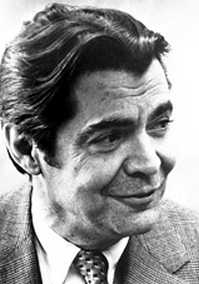
\includegraphics[width=0.30\textwidth]{11.jpg}} 
\subfloat[Vesicle Transport]{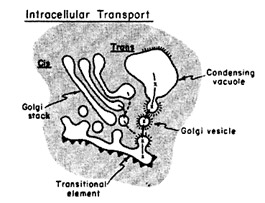
\includegraphics[width=0.56\textwidth]{55.jpg}} 
\caption{The concept of intracellular transport}
\label{some example}
\end{figure}
   \end{frame}

  
    \begin{frame}[label=simmonshall]{Machinery regulating vesicle traffic system (VTS) [2]}
    \begin{figure}
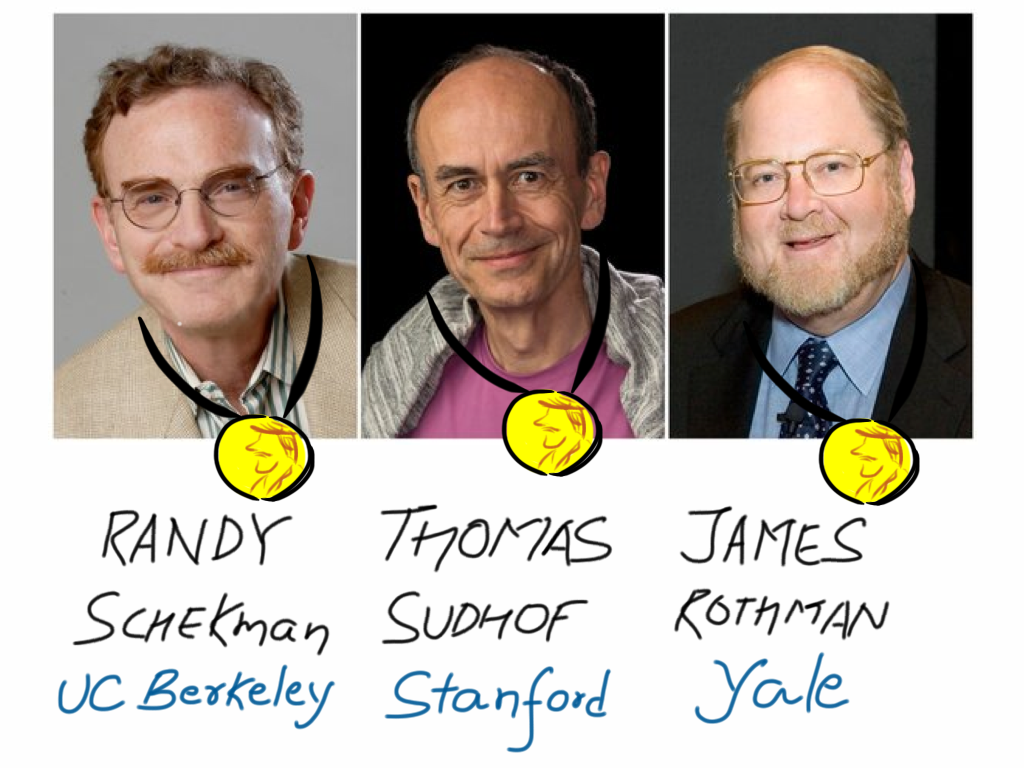
\includegraphics[width=0.35\textwidth]{22.png} 
\label{some example}
\end{figure}

      \begin{block}{Randy Schekman}
        Discovered set of \alert{genes}: required for vesicle traffic.
      \end{block}
      \begin{exampleblock}{James Rothman}
       \alert{Protein machinery}: allows vesicles to fuse with their
targets.
%to permit transfer of cargo.
      \end{exampleblock}
      \begin{alertblock}{Thomas Südhof}
        \alert{Signals} instruct vesicles to release their cargo with precision.
      \end{alertblock}
    \end{frame}
 
  
  \subsection{VTS to labeled Graph}
  
  \begin{frame}[label=figs1]{Cell as transport graph with pairing matrix}
    \begin{figure}
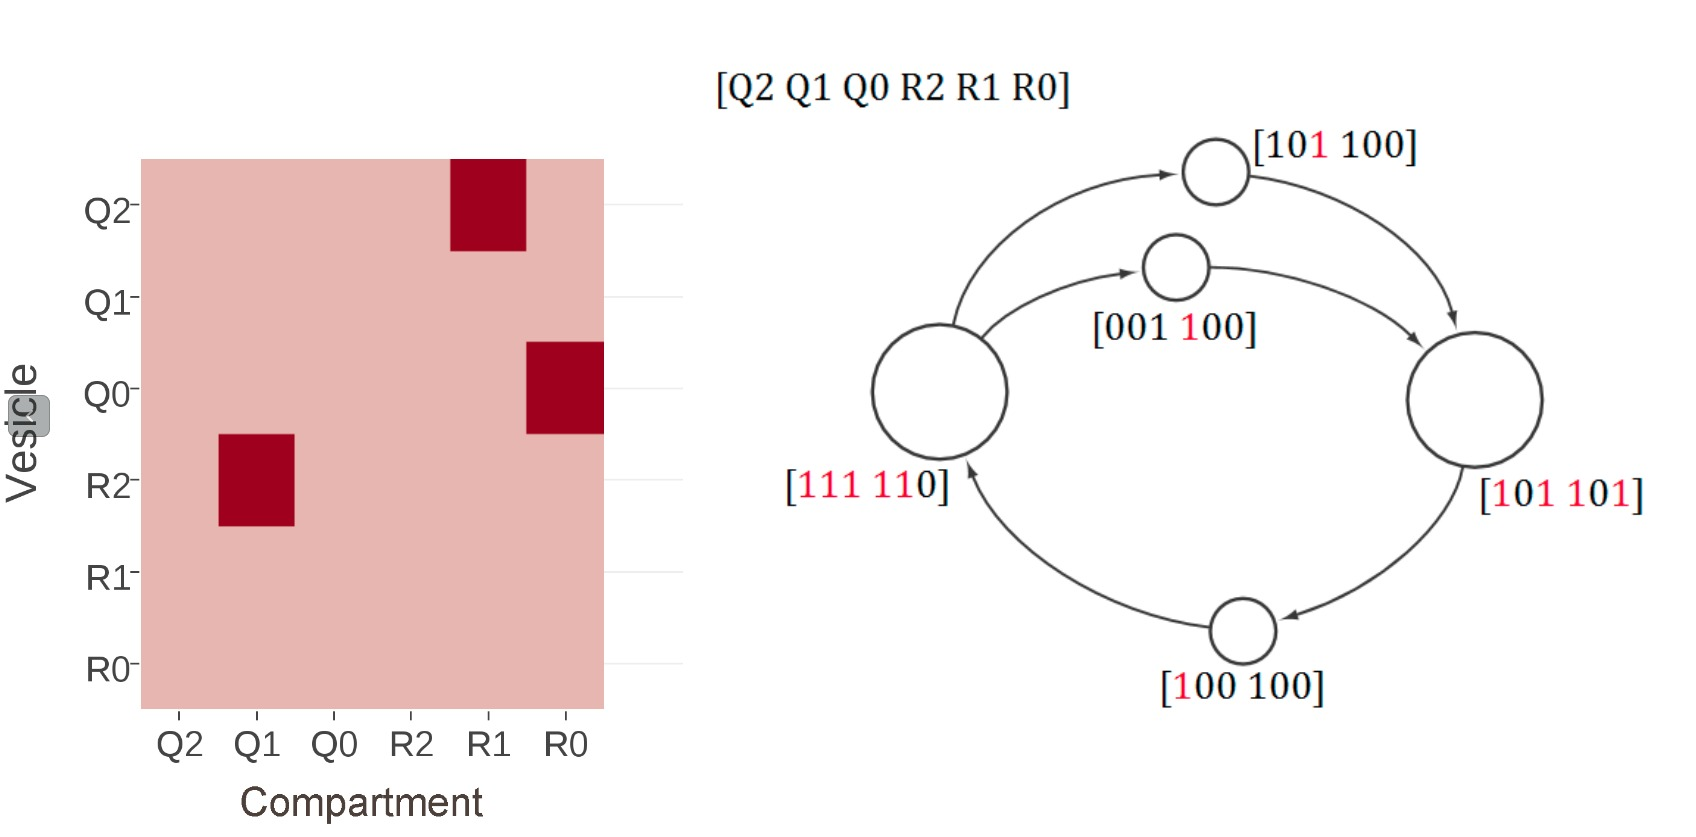
\includegraphics[width=0.90\textwidth]{3.jpg} 
\caption{VTS can be thought as a graph with compartment as nodes and vesicles as directed edges.}
\label{some}
\end{figure}
        \end{frame}
  
  \subsection{Queries over the model}
\defverbatim[colored]\sleepSort{     
\begin{lstlisting}[language=C,
mathescape,
  breaklines,
  frame=single,
  caption= Least connectivity property.,
] 
/* C1: Steady state condition.*/
/* C2, C3: Fusion rules.*/
/* C4: Graph is 4-connected.*/
/* G: Graph, f: Constrained function.*/
/* There exists a 4 connected graph for the given model.*/
SAT ( C1(G) $\wedge$ C2(G,f) $\wedge$ C3(G,f) $\wedge$ C4(G)) 
\end{lstlisting}

\begin{lstlisting}[language=C, 
mathescape, breaklines,	  frame=single,
  caption= Guaranteed connectivity property,
] 
/* C4: Graph is 4-connected.*/
/* G: Graph, f: Constrained function.*/
/* For every 4-connected graph this conditions must be valid.*/ 
VALID ($\forall$ G: C4(G) $\supset$ ($\exists$ f: C1(G) $\wedge$ C2(G,f) $\wedge$ C3(G,f) ))
\end{lstlisting} 
}  
   % \subsection{Queries on the model}
 \begin{frame}{Least connectivity and guaranteed connectivity [3].}
 {Connect Set of rules driving the VTS to graph connectivity.}
 \sleepSort
  \end{frame}
  
  
  
\defverbatim[colored]\sleepSort{
     
\begin{lstlisting}[language=C, mathescape,
  breaklines,	  frame=single,
  caption= Formally,
]
$  M , s \vDash f $ 
\end{lstlisting}}
        
  \subsection{Model checking }
 \begin{frame}{Model Checking [4-5]}{"Let M be a Kripke structure (i.e., state-transition graph). Let f be a formula of temporal logic (i.e., the specification)."}
  
\begin{equation}
  M , s \vDash f 
\end{equation}
 %\sleepSort
 \textbf{Model checking } or property checking refers to the following problem: Given a model of a system, exhaustively and automatically check whether this model meets a given specification
  
  \end{frame}
  
  
  
  \begin{frame}{CBMC, SAT, DPLL}{The tool is a bounded model checker; can check only finite length execution.}
  \begin{figure}
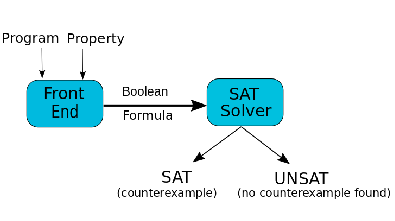
\includegraphics[width=0.65\textwidth]{6.png} 
\caption{CBMC: A Bounded model checker}
\label{some1}
\end{figure}
  \end{frame}   
  
  
    \begin{frame}[label=figs2]{Variations and corresponding graph connectivity}
 \begin{table}[!b]       
      
      \end{table}
\end{frame}


\subsection{Encoding the SSC and Fusion rules}
 \defverbatim[colored]\sleepSort{
     
 \begin{lstlisting}[language=haskell,
mathescape,
 breaklines,
  frame=single,
  caption= Steady state specification,
]
-- E(x,y): Edge between node x and y. E.source = x, E.target = y    
-\end{l- Edge(m)(x,y): Edge between node x and y with labelE(m).                 

$\forall$ z $\in$ {Nodes} $\forall$ E $\in$ {Edges}: E.source = z $\supset$
    $\forall$ m $\in$ {Molecules}: labelE(m) $\supset$
       ($\exists$ a seq(a1..an): (2 $\leq$ |seq| $\leq$ N)  $\wedge$
            ((a1 = z) $\wedge$ (a2 = E.target) $\wedge$
             (($\forall$ k from 1 to |seq| - 1) $\supset$  Edge(m)(ak,ak+1)) $\wedge$
             (Edge(m)(an,a1)))

\end{lstlisting}
}

    \begin{frame}{Steasy state condition:}{The VTS is said to be in steady state if every molecule leaving the nodes comes back to its source node in a cycle.}
    
      \sleepSort
    \end{frame}



    \defverbatim[colored]\sleepSort{
      \begin{lstlisting}[language=C,tabsize=2]
  

/* Declare an arbitrary unsigned integer big. */            
 unsigned int hop;

/* Constraint it represent(mentally) N-2 hops. */
 __CPROVER_assume( hop >= 1 && hop <= (N - 2));
    
/* An array to store the path taken by molecule. */
 unsigned int path[hop];   
 
/* Make sure each index stores a node. */
 for (l = 0 to hop) {           // Dynamic
     path[l] = zeroTon(N - 1);
 }
\end{lstlisting}}

    \begin{frame}{Code listings}{Non-determinism and enumeration}
      \sleepSort
    \end{frame}
    
\defverbatim[colored]\sleepSort{
\begin{lstlisting}[mathescape, language=C,
  frame=single,
  caption= Edge respects fusion rules,
]
# ActiveE(i): ith molecule is active on edge E. 
# ActiveY(j): jth molecule is active on node y.
$\forall$ x,y $\in$ {Nodes}: E(x,y) $\supset$
($\exists$i,j $\in$ [1..M]: ActiveE(i) $\wedge$  ActiveY(j)
                           $\wedge$ (pairingMatrix(i,j) = 1)) 
\end{lstlisting}

\begin{lstlisting}[mathescape,language=C,
  frame=single,
  caption= Two edges of identical composition should go to the same target,
]
# labelE: label of edge E.
(labelE = labelE$^{\prime}$) $\supset$ (E.target = E$^{\prime}$.target) 

\end{lstlisting}

\begin{lstlisting}[mathescape,language=C,
  frame=single,
  caption= Graph topology is respected,
]
$\forall$ x,y,z $\in$ {Nodes}: E(x,y)
($\forall$i,j $\in$ [1..M] (ActiveE(i) $\wedge$  ActiveZ(j) $\wedge$ 
                pairingMatrix(i,j) = 1) $\supset$ (z = y))
\end{lstlisting}
}

    \begin{frame}{Fusion rules}{}
      \sleepSort
    \end{frame}
  
% \begin{lstlisting}[language=haskell,caption= Steady state condition, 
% mathescape,
%   breaklines,
%   rulecolor=\color{black},
%   frame=single
% ]
% -- edge_m(x,y): There is an edge between node x and y, and molecule m is  present on that edge.
% -- seq(a1..1n): each ai represents a node.

% $\forall$ n $\in$ {Node}
%  $\forall$ e $\in$ {Edges}: e.source == n
%    $\forall$ m On e
%     $\exists$
%        an edge(i,j)
%      Or
%        a seq(1..k): |seq| $\leq$ N - 2
%          edge(e.target,seq(1)) && edge_m(seq(1),seq(2)) 
%          && ... && edge(seq(k),e.source)
% }
% \end{lstlisting}



\begin{frame}{Scalability}{Improved by not upto the required level}
We were able to scale to N = 8 (Total 8 compartments and 36 molecules). 
\end{frame} 

\section{Encoding directly under the solver: Tool MAA}

  \begin{frame}[label=proof]{Reachability and steady state Rules of VTS}
    We use reachability to encode the stability condition in VTSs.
  %    \framesubtitle{All integers divide zero}
      \begin{definition}
        $\bigwedge\limits_{i,j,m,p} r_{i,j,m,p} \implies (\, e_{i,j,m} \lor \bigvee_{i\neq i^{\prime}} ( \, e_{i,i^{\prime},m} \land r_{i^{\prime},j,m,p-1} ) )$
      \end{definition}
      \begin{theorem}
        $\bigwedge\limits_{i,j,m} ( e_{i,j,m} \implies r_{j,i,m,\mu})$
      \end{theorem}
%       \begin{proof}[Proof\nopunct]
%         $\forall a\in\mathds{Z}: a\cdot 0=0$
%       \end{proof}
    \end{frame}
    
    \subsection{Reachability encoding}


    \subsection{Queries revisited}
    \begin{frame}[label=math]{$k$-connectivity constraints}
    The following constraints encode that only
existing edges can be dropped and exactly $k-1$ edges are dropped.
     \begin{equation}
\begin{alignedat}{2}
\ \bigwedge\limits_{i,j} d_{i,j} \implies e_{i,j}\\
  \sum_{i,j} d_{i,j} = k-1
\end{alignedat}
\end{equation}
but, in my opinion, the following is better
\begin{equation}
\begin{alignedat}{2}
\bigwedge\limits_{i,j}  [(e_{i,j} \land  \neg d_{i,j}) \lor  (\bigvee_{i' \neq i}  r^{\prime}_{i',j} \land  (e_{i,i'} \land \neg d_{i,i'}) ] \implies r^{\prime}_{i,j}  
\end{alignedat}
\end{equation}

 \begin{equation}
\begin{alignedat}{2}
 \bigvee\limits_{i,j} \neg (r^{\prime}_{i,j} \lor r^{\prime}_{j,i})
\end{alignedat}
\end{equation}
\end{frame}
  
  
  \defverbatim[colored]\sleepSort{


\begin{lstlisting}[language=C, 
mathescape, breaklines,	  frame=single,
  caption= Guaranteed connectivity property,
] 
/* C4: Graph is 4-connected.*/
/* G: Graph, f: Constrained function.*/
/* For every 4-connected graph this conditions must be valid.*/ 
VALID ($\forall$ G: C4(G) $\supset$ ($\exists$ f: C1(G) $\wedge$ C2(G,f) $\wedge$ C3(G,f) )) 

\end{lstlisting} 
    
}

    \begin{frame}{Quantifiers over boolean function !!}{Guarantee connectivity revisited.}
      \sleepSort
    \end{frame}
    
    \subsection{Quantifier elimination}
\begin{frame}{Qunatifier elimination}{Advanced techniques}
\begin{enumerate}
\item Skolemize
\item David Monerix
\item Synthesis problem
\end{enumerate}
\end{frame}

%     \subsection{Citations and Bibliography}
%     \begin{frame}[label=citations]{Citations}
%       \framesubtitle{\TeX, \LaTeX, and Beamer}

%       \justifying\TeX\ is a programming language for the typesetting
%       of documents. It was created by Donald Erwin Knuth in the late
%       1970s and it is documented in \emph{The \TeX
%       book}~\cite{knuth84}.

%       In the early 1980s, Leslie Lamport created the initial version
%       of \LaTeX, a high-level language on top of \TeX, which is
%       documented in \emph{\LaTeX : A Document Preparation
%       System}~\cite{lamport94}. There exists a healthy ecosystem of
%       packages that extend the base functionality of \LaTeX;
%       \emph{The \LaTeX\ Companion}~\cite{MG94} acts as a guide
%       through the ecosystem.

%       In 2003, Till Tantau created the initial version of Beamer, a
%       \LaTeX\ package for the creation of presentations. Beamer is
%       documented in the \emph{User's Guide to the Beamer
%       Class}~\cite{tantau04}.
%     \end{frame}

    \begin{frame}[label=bibliography]{Bibliography}
      \framesubtitle{\TeX, \LaTeX, and Beamer}
      \begin{thebibliography}{9}
      \bibitem{palade75}
      Palade~George. 
      \emph{Intracellular aspects of the process of protein synthesis.}
      Science 189.4200 (1975): 347-358.
      
      \bibitem{rothman14}
      Rothman~James~Edward. 
      \emph{Principle of membrane fusion in the cell (Nobel lecture).}
      Angewandte Chemie International Edition 53.47 (2014): 12676-12694.
      
      \bibitem{shukla17}
      Shukla~Ankit, et al. 
      \emph{Discovering vesicle traffic network constraints by model checking.}
      PloS one 12.7 (2017): e0180692.
      
      \end{thebibliography}
    \end{frame}

%   \section{Dark Frames}
%    \begin{darkframes}
%     \end{darkframes}
%    \subsection{Blind Text}
%     \begin{frame}{Jabberwocky}
%       \framesubtitle{Lewis Carroll}%
%       \begin{tikzpicture}[overlay,remember picture]
%         \node[anchor=south east,xshift=-30pt,yshift=35pt]
%           at (current page.south east) {
%             
\includegraphics[width=35mm]{resources/jabberwocky-dark}
%           };
%       \end{tikzpicture}%
%       'Twas brillig, and the slithy toves\\
%       Did gyre and gimble in the wabe;\\
%       All mimsy were the borogoves,\\
%       And the mome raths outgrabe.\\\bigskip

%       “Beware the Jabberwock, my son!\\
%       The jaws that bite, the claws that catch!\\
%       Beware the Jubjub bird, and shun\\
%       The frumious Bandersnatch!”\\
%     \end{frame}
% %     \againframe{lists}
%     \subsection{Structuring Elements}
%     \againframe{simmonshall}
%     \againframe{proof}
%     \subsection{Numerals and Mathematics}
%     \againframe{math}
%     \subsection{Figures and Code Listings}
%     \againframe{figs1}
%     \againframe{figs2}
%     \defverbatim[colored]\sleepSort{
%       \begin{lstlisting}[language=C,tabsize=2]
% #include <stdio.h>
% #include <unistd.h>
% #include <sys/types.h>
% #include <sys/wait.h>

% // This is a comment
% int main(int argc, char **argv)
% {
%         while (--c > 1 && !fork());
%         sleep(c = atoi(v[c]));
%         printf("%d\n", c);
%         wait(0);
%         return 0;
% }
%     \end{lstlisting}}
%   \begin{frame}{Code listings}{An example source code in C}
%       \sleepSort
%     \end{frame}
%     \subsection{Citations and Bibliography}
%     \againframe{citations}
%     \againframe{bibliography}
 % \end{darkframes}
 
 
\end{document}
